\documentclass[a4paper,11pt]{book}

\usepackage{amsmath}
\usepackage{amssymb}
\usepackage[amssymb]{SIunits}
\usepackage{graphicx}
\usepackage[table]{xcolor}
\usepackage{enumitem}
\usepackage{fancyhdr}
\usepackage[footnotesize,bf]{caption}
\usepackage{sidecap}
% \usepackage{longtable}
% \usepackage{multirow}
% \usepackage{booktabs}
\usepackage[pdfborder={0 0 0}]{hyperref}
% \usepackage{float}

% \usepackage{titlesec}
% \titleformat{\chapter}[hang]{\bf\huge}{\thechapter}{0.5em}{}
% \titlespacing{\chapter}{0pt}{0pt}{50pt}

\usepackage{natbib}
\setlength{\bibsep}{1pt}
\renewcommand{\bibfont}{\footnotesize}

\hoffset -1in
\voffset -1in

\topmargin      10mm
\headheight     10mm
\headsep        10mm
\oddsidemargin  25mm
\textwidth     160mm
\textheight    242mm

%\title{\bf DNS/TMP User Guide}
\title{{\bf AT}\textcolor{black!50}{Lab} Documentation}
\author{Turbulence and Boundary Layers Group $|$ University of Hamburg}

\setcounter{tocdepth}{2}
\setlength{\parindent}{0mm}

\fancyhead[LE,LO]{\footnotesize\leftmark}
\fancyhead[RE,RO]{}

%%%%%%%%%%%%%%%%%%%%%%%%%%%%%%%%%%%%%%%%%%%%%%%%%%%%%%%%%%%%%%%%%%%%%%
\def\pst{\partial_t}
\def\psk{\partial_k}

\def\Re{\mathrm{Re}}
\def\Pr{\mathrm{Pr}}
\def\Sc{\mathrm{Sc}}
\def\Fr{\mathrm{Fr}}
\def\Ro{\mathrm{Ro}}
% \def\Le{\mathrm{Le}}
% \def\Ma{\mathrm{Ma}}
% \def\Da{\mathrm{Da}}

\def\j{\mathbf{j}}
\def\e{\mathbf{e}}

\def\bg{_\mathrm{bg}}
\def\ss{_\mathrm{s}}
\def\sc{_\mathrm{c}}

\newcommand{\pt}[2] {\partial_{#2}{#1}}
\newcommand{\ptp}[2]{\partial_{#2}\left(#1\right)}
% \newcommand{\ptp}[1]{\partial_t\left(#1\right)}
% \newcommand{\pjp}[1]{\partial_j\left(#1\right)}
\newcommand{\dvp}[1]{\nabla\negmedspace\cdot\negthinspace\left(#1\right)}
\newcommand{\dv} [1]{\nabla\negmedspace\cdot\negthinspace#1}
\newcommand{\avr}[1]{\overline{#1}}
\newcommand{\avf}[1]{\widetilde{#1}}


%%%%%%%%%%%%%%%%%%%%%%%%%%%%%%%%%%%%%%%%%%%%%%%%%%%%%%%%%%%%%%%%%%%%%%
\begin{document}

\frontmatter
\pagestyle{empty}
\maketitle
\tableofcontents

\setlength{\parskip}{0.5\baselineskip}
%\include{preface}

\chapter*{Preface}
\addcontentsline{toc}{chapter}{Preface}
\sloppy

ATLab---an acronym for Atmospheric Turbulence Laboratory---is a set of tools whose aim is {\bf to efficiently solve and analyze a particular set of governing equations with a controlled accuracy}. The accuracy can be controlled in different ways: comparing with analytical solutions, including linear stability analysis; grid convergence studies; balance of transport equations, like integral turbulent kinetic energy or local values at specific relevant locations (e.g., at the wall). Resolution can be measured by the ratio between the grid spacing $\Delta x$ and the relevant small scales, like the Kolmogorov scale $\eta$ or the thickness of the diffusion sub-layers next to the wall. For the compact schemes used here, typical values are $\Delta x/\eta\simeq 1-2$; larger values can lead to numerical instability because of the aliasing generated by the non-linear terms. Note that these schemes are non-monotone, but typical out-of-bounds deviations of conserved scalars are below $10^{-6}-10^{-8}$ relative to the mean variations, and this error is therefore negligibly small compared to the typical error associated with the statistical convergence, of the order of $1-5$\%. The statistical convergence can be estimated by varying the sample size of the data set, e.g. varying the domain size along the statistically homogeneous directions. 

The efficiency can be measured in different ways but, ultimate, it should be related with the computational time needed to understand a particular problem with a given accuracy, and so the importance of the controlled accuracy. 

Making the code user-friendly comes after the previous two main priorities: controlled accuracy and efficiency.

Last, the main documentation is the code itself and the examples. This document is only a short introduction to the equations and the tools. The code is continuously under development, so this document is continuously incomplete.

\mainmatter
\pagestyle{fancy}

\part{User Guide}
\def\pt{\partial_t}
\def\psi{\partial_i}
\def\pk{\partial_k}

\def\Re{\mathrm{Re}}
\def\Pr{\mathrm{Pr}}
\def\Sc{\mathrm{Sc}}
\def\Fr{\mathrm{Fr}}
\def\Ro{\mathrm{Ro}}
% \def\Le{\mathrm{Le}}
% \def\Ma{\mathrm{Ma}}
% \def\Da{\mathrm{Da}}

\def\j{\mathbf{j}}
\def\e{\mathbf{e}}

\def\ref{_\mathrm{bg}}
\def\ss{_\mathrm{s}}
\def\sc{_\mathrm{c}}

\chapter{Governing equations}\label{sec:equations}

The code is build to solve the sets of equations described in this section as efficiently as possible. These sets of equations aim to be general enough to cover several problems. The consequence is that one needs to map the particular problem to one of these generic cases, and identify the appropriate values of the parameters and defining functions (for instance, $\Re$ or $b^e$). Certain knowledge of the equations is therefore advantageous.

%%%%%%%%%%%%%%%%%%%%%%%%%%%%%%%%%%%%%%%%%%%%%%%%%%%%%%%%%%%%%%%%%%%%%%%%%%%%%%%%
\section{Evolution equations}

\subsection{Boussinesq}

Dynamics and thermodynamics are at most coupled by the buoyancy field, and thermodynamics is not necessary (but can still be used). We consider the momentum equation and the evolution equations for an arbitrary number of scalar fields in the following form:
\begin{subequations}
    \begin{align}
        &\pt v_i = -v_k\pk v_i + \pk\left(\Re^{-1} \nu \pk v_i\right) -\psi p'
        +\Fr^{-1} g_i\,b +\Ro^{-1}\,\epsilon_{ijk} f_k\,v_k\;, &&i =1,2,3 \\
        &\pt s_i  = -v_k\pk s_i +\pk \left[(\Re\Sc_i)^{-1} \nu \pk s_i -\pk (\j_i)_k\right] + \omega_i \;, &&i = 1,\ldots\,n
    \end{align}
\end{subequations}
The dynamic variables in these equations are  nondimensionalized by $\rho_0$, $U_0$ and $L_0$. The parameters $\Re$, $\Sc$, $\Fr$ and $\Ro$ need to be provided.
\begin{itemize}
    \item The scalar field $\nu$ represents the kinematic viscosity. In the simplest case, it is equal to 1.
    \item The scalar field $b$ represents the buoyancy, if any. The vector $(g_i)$ gives the direction of the buoyancy force and it is constant.
    \item The vector fields $\j_i$ represent flux terms, if any.
    \item The scalar fields $\omega_i$ represent source terms, if any.
\end{itemize}
These fields are defined in terms of the scalars $s_k$ by functions $\nu^e(s_k)$, $b^e(s_k)$, $\j^e_i(s_k)$ and $\omega^e_i(s_k)$, to be given.
\begin{itemize}
    \item The vector $(f_i)$ gives the direction of the angular velocity of the frame of reference, if any. It is assumed constant.
\end{itemize}
Mass conservation,
\begin{equation}
    \pk v_k=0\;,
\end{equation}
is imposed in terms of the pressure-Poisson equation
\begin{equation}
    \nabla^2 p'=\pk(\ldots)
\end{equation}
with the boundary conditions that result from particularizing the momentum equation at the top and bottom boundaries. Details can be found in \cite{mellado2012factorization}.

\subsubsection{Dimensional Formulation}

A dimensional formulation can be considered by substituting the parameters \texttt{Reynolds}, \texttt{Froude} and \texttt{Rossby} the input file (by default, \texttt{tlab.ini}) with \texttt{Viscosity}, \texttt{Gravity} and \texttt{Coriolis}. The boundary and initial conditions defined in the input file should then be given in dimensional form. 

\subsection{Anelastic}

Dynamics and thermodynamics are coupled by the density. The momentum equation is formulated in terms of the dynamic pressure and the density:
\begin{equation}
    \pt v_i = -v_k\pk v_i + \rho\ref^{-1}\pk\left(\Re^{-1} \mu \pk v_i\right) -\rho\ref^{-1}\psi p'
        +\Fr^{-1} g_i(1-\rho/\rho\ref)+\Ro^{-1}\,\epsilon_{ijk} f_k\,v_k\;.
\end{equation}
The evolution equations for the scalars read:
\begin{equation}
    \pt s_i  = -v_k\pk s_i +\rho\ref^{-1}\pk \left[(\Re\Sc_i)^{-1} \mu \pk s_i -\pk (\j_i)_k\right] + \omega_i \;, \qquad i = 1,\ldots\,n
\end{equation}
Symbols are as explained in the Boussinesq case. The scalar field $\mu$ represents the dynamic viscosity. In the simplest case, it is equal to 1.
\par
Mass conservation,
\begin{equation}
    \pk (\rho\ref v_k)=0\;,
\end{equation}
is imposed in terms of the pressure-Poisson equation
\begin{equation}
    \nabla^2 p'=\pk(\rho\ref \ldots)
\end{equation}
with the boundary conditions that result from particularizing the momentum equation at the top and bottom boundaries

\subsection{Compressible}

Dynamics and thermodynamics are fully coupled. The pressure in the momentum equation is the thermodynamic pressure. Mass conservation is expressed in terms of the evolution equation
\begin{equation}
    \pt \rho = -\pk(\rho v_k) 
\end{equation}
instead of a solenoidal constraint.

The variables in these equations are normalized by the reference scales $\mathrm{L}_0$, $\mathrm{U}_0$, $\rho_0$ and $\mathrm{T}_0$, which represent a length, a velocity, a density, and a temperature, respectively. The pressure is normalized by $\rho_0U_0^2$. 

TBD

%%%%%%%%%%%%%%%%%%%%%%%%%%%%%%%%%%%%%%%%%%%%%%%%%%%%%%%%%%%%%%%%%%%%%%%%%%%%%%%%
\section{Thermodynamics}

We consider $n\sc$ components (or species) with mass fractions $\zeta_i$.

\subsection{Compressible}
The thermal equation of state is implemented as
\begin{equation}
    p = \rho R T \;.
\end{equation}
The scalar field 
\begin{equation}
    R =\sum^{n\sc}_1 R_i\zeta_i
\end{equation}
is the specific gas constant of the mixture.

The caloric equation of state is implemented as
\begin{equation}
    h = \sum^{n\sc}_1 h_{i} \zeta_i \;,\qquad h_{i} = \Delta h^0_i + \int^{T}_{T_0}
    c_{pi}(T) dT \;.
\end{equation}

Each species has a specific heat capacity $c_{pi}$ and a specific gas constant $R_i=\mathcal{R}/W_i$,  where  $\mathcal{R}$ is the universal gas constant and $W_i$ the molar mass of the species. They are nondimensionalized by the reference values $c_{p0}$ and $R_0=\mathcal{R}/W_0$, respectively, which are the values of one of the species. %They are defined in the procedure \texttt{Thermodynamics\_Initialize}. 

The thermodynamic variables are nondimensionalized as in evolution equations, i.e., the reference scales $\mathrm{L}_0$, $\mathrm{U}_0$, $\rho_0$ and $\mathrm{T}_0$, which represent a length, a velocity, a density, and a temperature, respectively. The pressure is normalized by $\rho_0U_0^2$. Thermal energy variables are normalized with $c_{p0}T_0$, where $c_{p0}$ is a reference specific heat capacity at constant pressure.

TBD

\subsubsection{Dimensional Formulation}

In this case of a multi-species, a dimensional formulation can be considered by setting the input parameter \texttt{nondimensional} equal to \texttt{.false.} in the block \texttt{[Thermodynamics]} of the input file (by default, \texttt{tlab.ini}). 

\subsection{Anelastic}
The thermal equation of state is implemented as
\begin{equation}
    p\ref = \rho R T \;.
\end{equation}
The thermodynamic variables are nondimensionalized by $\rho_0$, $T_0$ and $R_0$, such that $p_0=\rho_0R_0T_0$. The default reference values are $p_0=10^5$~Pa and $T_0=298$~K. Thermal energy variables are normalized with $c_{p0}T_0$, where $c_{p0}$ is a reference specific heat capacity at constant pressure.

The caloric equation of state is formulated in terms of the static energy
\begin{equation}
    h =\sum^{n\sc}_1 h_{i} \zeta_i + \frac{\gamma_0-1}{\gamma_0}H^{-1}(x_3-x_{3,0}) \;.
\end{equation}
The scalar field $c$ is the specific heat capacity, a function of the scalars $s_i$. The parameter
\begin{equation}
    H = \frac{R_0T_0}{gL_0}
\end{equation}
is a nondimensional scale height, or the inverse of a nondimensional gravity, to be provided. The parameter
\begin{equation}
    R_0/c_{p0} =(\gamma_0-1)/\gamma_0 \;,
\end{equation}
a conversion factor between gas constants and heat capacities (thermal equation of state and caloric equation of state). We refer to it in the code as \texttt{GRATIO}. 

The background profiles $\{\rho\ref,\, p\ref,\, T\ref,\, \zeta_{i,\mathrm{ref}}\}$ correspond to a state of thermodynamic and hydrostatic equilibrium. The code solves the system of equations
\begin{subequations}
    \begin{align}
        &\partial_3\,p\ref=-H^{-1}\, g_3\,\rho\ref\;,\qquad p\ref|_{x_3=x_{3,0}}=p_{\mathrm{bg},0}\;,\\
        &p\ref  = \rho\ref R\ref T\ref \;.
    \end{align}
\end{subequations}
$\mathbf{g}$ is defined opposite to the gravitational acceleration (the problem is formulated in terms of the buoyancy). The two equations above relate 4 thermodynamic variables and we need two additional constraints. Typically, we impose the background profile of static energy (enthalpy plus potential energy) and the composition. If there is only one species, then $R\ref=1$ and we only need one additional constraint. 

Currently implemented only for air-water mixtures. In this case, the first scalar is the energy variable and the remaining scalars are the composition (e.g., total water specific humidity and liquid water specific humidity).

\subsubsection{Dimensional Formulation}

A dimensional formulation can be considered by setting the parameter \texttt{nondimensional} equal to \texttt{.false.}, which sets \texttt{GRATIO} equal to 1

\subsection{Mixtures}

We consider $n\sc$ components (or species) with mass fractions $\zeta_i$. These need not be equal to the prognostic scalar variables $s_k$, and the relationship between them $\zeta_i=\zeta_i^e(s_k)$ needs to be given.

In the generic case, we choose
\begin{equation}
    \zeta_i=s_i\;,\quad i=1,\ldots,n\sc-1\;,
\end{equation}
and the last component has a mass fraction
\begin{equation}
    \zeta_{n\sc} = 1-\sum_1^{n\sc-1}\zeta_i \;.
\end{equation} 
The gas constant can then be written as 
\begin{equation}
    R=\sum_1^{n\sc}\zeta_iR_i=\sum_1^{n\sc-1}(R_i-R_N) \;,
\end{equation}
and similarly for other thermodynamic variables.

Particular cases different from this one occur for instance when we consider chemical equilibrium or phase equilibrium, or when different combinations of mass fractions might be preferable to better represent conservation properties.

%For instance, in the case of moist thermodynamics with phase equilibrium (saturation adjustment), only the total water content is a prognostic variables and the partition into liquid and vapor is done assuming phase equilibrium.

\subsubsection{Air-water mixtures in anelastic formulations}

We consider the total water specific humidity as prognostic variable. If necessary, we also consider the liquid water specific humidity, which can be diagnostic in the case of phase equilibrium, or prognostic otherwise.


% %%%%%%%%%%%%%%%%%%%%%%%%%%%%%%%%%%%%%%%%%%%%%%%%%%%%%%%%%%%%%%%%%%%%%%%%%%%%%%%%
% \section{Dimensional formulations}


% \include{bcs}
% \include{code}
% \include{grid}
\chapter{Post-Processing Tools}\label{sec:postprocessing}

%%%%%%%%%%%%%%%%%%%%%%%%%%%%%%%%%%%%%%%%%%%%%%%%%%%%%%%%%%%%%%%%%%%%%%%%%%%%%%%%
%%%%%%%%%%%%%%%%%%%%%%%%%%%%%%%%%%%%%%%%%%%%%%%%%%%%%%%%%%%%%%%%%%%%%%%%%%%%%%%%
\section{Averages}

See file {\tt dns/tools/postprocessing/averages}.

Allows for conditional analysis.

% %%%%%%%%%%%%%%%%%%%%%%%%%%%%%%%%%%%%%%%%%%%%%%%%%%%%%%%%%%%%%%%%%%%%%%%%%%%%%%%%
% %%%%%%%%%%%%%%%%%%%%%%%%%%%%%%%%%%%%%%%%%%%%%%%%%%%%%%%%%%%%%%%%%%%%%%%%%%%%%%%%
% \section{Probability density functions}

% See file {\tt dns/tools/postprocessing/pdfs}.

% Allows for conditional analysis.

% %%%%%%%%%%%%%%%%%%%%%%%%%%%%%%%%%%%%%%%%%%%%%%%%%%%%%%%%%%%%%%%%%%%%%%%%%%%%%%%%
% %%%%%%%%%%%%%%%%%%%%%%%%%%%%%%%%%%%%%%%%%%%%%%%%%%%%%%%%%%%%%%%%%%%%%%%%%%%%%%%%
% \section{Conditional analysis}

% To be developed.

% %%%%%%%%%%%%%%%%%%%%%%%%%%%%%%%%%%%%%%%%%%%%%%%%%%%%%%%%%%%%%%%%%%%%%%%%%%%%%%%%
% %%%%%%%%%%%%%%%%%%%%%%%%%%%%%%%%%%%%%%%%%%%%%%%%%%%%%%%%%%%%%%%%%%%%%%%%%%%%%%%%
% \section{Two-point statistics}
% \sloppy

% See file {\tt dns/tools/postprocessing/spectra}. Based on package FFTW \cite{frigo2005design}.

% Given two scalar fields $\{a_{nm}:\,n=1,\ldots,N,\,m=1,\ldots,M\}$ and similarly $b_{nm}$, we calculate the one-dimensional co-spectra $\{E^x_0,\,E^x_1,\,\ldots,\,E^x_{N/2}\}$ and $\{E^z_0,\,E^z_1,\,\ldots,\,E^z_{M/2}\}$ normalized such that \begin{equation} \langle ab\rangle = E^x_0+2\sum_1^{N/2-1}E^x_n+E^x_{N/2} = E^z_1+2\sum_0^{M/2-1}E^z_m+E^z_{M/2} \end{equation} The mean value is removed, such that the left-hand side is $\langle a'b'\rangle$. The Nyquist frequency energy content $E^x_{N/2}$ and $E^z_{M/2}$ is not written to disk, only the $N/2$ values $\{E^x_0,\,E^x_1,\,\ldots,\,E^x_{N/2-1}\}$ and the $M/2$ values $\{E^z_0,\,E^z_1,\,\ldots,\,E^z_{M/2-1}\}$. When $a\equiv b$, then we obtain the power spectral density.

% The sum above can be interpreted as the trapezoidal-rule approximation to the integral $(L/2\pi)\int_0^{\kappa_c}2E(\kappa)\mathrm{d}\kappa$, where $\kappa_c=\pi/h$ is the Nyquist frequency, $\Delta \kappa=\kappa_c/(N/2)=2\pi/L$ is the uniform wavenumber spacing, $h=L/N$ is the uniform grid spacing and $L$ is the domain size. Hence, the physical spectral function at wavenumber $\kappa_n= n\Delta \kappa$ (equivalently, wavelength $L/n$) is $2E_n/\Delta \kappa$.

% Due to the relatively large size of the files, we split the calculations is the auto-spectra and the cross-spectra. The corresponding files containing the one-dimensional spectra along the direction $Ox$ are {\tt xsp} and {\tt xCsp}, respectively, and similarly along the direction $Oz$. The two-dimensional co-spectra $E_{nm}$ can also be written to disk, though the additional memory requirement can be a difficulty.

% The one-dimensional cross-correlations $\{C^x_0,\,C^x_1,\,\ldots,\,C^x_{N-1}\}$ and $\{C^z_0,\,C^z_1,\,\ldots,\,C^z_{M-1}\}$ are normalized by $a_\mathrm{rms}b_\mathrm{rms}$, so that $C^x_0 = C^z_0 =1$ when $a\equiv b$ and we calculate the auto-correlations. The auto-correlations are even functions and therefore only $\{C^x_0,\,C^x_1,\,\ldots,\,C^x_{N/2-1}\}$ and $\{C^z_0,\,C^z_1,\,\ldots,\,C^z_{M/2-1}\}$ are written to disk (note that we also dropped the last term $C^x_{N/2}$ and $C^z_{M/2}$.)

% The corresponding files containing the one-dimensional cross-correlations along the direction $Ox$ are {\tt xcr} and {\tt xCcr}, and similarly along the direction $Oz$. The two-dimensional cross-correlation $C_{nm}$ can also be written to disk, though the additional memory requirement can be a difficulty.

% Both form a Fourier pair according to
% \begin{equation*}
%     E_k=\frac{1}{N}\sum_0^{N-1}(a_\mathrm{rms}b_\mathrm{rms}C_n)\exp(-i\omega_kn)\;,\qquad
%     a_\mathrm{rms}b_\mathrm{rms}C_n=\sum_0^{N-1}E_k\exp(i\omega_kn)\;,
% \end{equation*}
% where $\{\omega_k=(2\pi/N)k:\, k = 0,\ldots,N-1\}$ is the scaled wavenumber and
% $i=\sqrt{-1}$ is the imaginary unit. Therefore,
% \begin{equation}
%     \frac{1}{N}\sum_0^{N-1}C_n=\frac{E_0}{a_\mathrm{rms}b_\mathrm{rms}} \;,
% \end{equation}
% relation that can be used to relate integral scales $\ell$ to the Fourier mode $E_0$, as follows. First, for the auto-correlation function, we can re-write
% \begin{equation}
%     \frac{1}{N/2}\sum_0^{N/2-1}C_n=\frac{E_0}{a_\mathrm{rms}^2}+\frac{1-C_{N/2}}{N}
% \end{equation}
% because
% \begin{equation*}
%     \frac{1}{N}\sum_0^{N-1}C_n = \frac{1}{N}\left(\sum_0^{N/2-1}C_n
%     +C_{N/2}+\sum_{N/2+1}^{N-1}C_n\right) = \frac{1}{N}\left(2\sum_0^{N/2-1}C_n
%     +C_{N/2}-1\right) \;,
% \end{equation*}
% since, from periodicity, $C_N=C_0=1$ and, from the symmetry of the auto-correlation sequence, $\sum_{N/2+1}^{N}C_n=\sum_0^{N/2-1}C_n$. Therefore, if we use a trapezoidal rule to define the integral length scale as
% \begin{equation}
%     \ell=h\left(\frac{C_0+C_{N/2-1}}{2}+\sum_1^{N/2-2}C_n\right)\;,
% \end{equation}
% where $h=L/N$ is the grid spacing and $L$ is the domain size, we obtain
% \begin{equation}
%     \ell=\frac{L}{2}\left(\frac{E_0}{a_\mathrm{rms}^2}-\frac{2C_{N/2}}{N}\right)
%     \simeq \frac{L}{2a_\mathrm{rms}^2}E_0\;.
% \end{equation}
% This result applies to both directions $Ox$ and $Oz$, providing relations between $\ell^x$ and $E^x$, and $\ell^z$ and $E^z$. Each case needs to use the corresponding domain size, $L^x$ and $L^z$.

% These relations show that the integral length scales can be obtained directly from the spectral information without the need to calculate the correlation functions. However, the statistical convergence of those integral scales might be too poor and alternative definitions might be more useful. Also, correlation functions provide information about the degree of de-correlation achieved with a particular domain size, and about the structural organization of the flow in terms of different properties.

%%%%%%%%%%%%%%%%%%%%%%%%%%%%%%%%%%%%%%%%%%%%%%%%%%%%%%%%%%%%%%%%%%%%%%%%%%%%%%%%
%%%%%%%%%%%%%%%%%%%%%%%%%%%%%%%%%%%%%%%%%%%%%%%%%%%%%%%%%%%%%%%%%%%%%%%%%%%%%%%%
\section{Summary of budget equations for second-order moments}

Let $f$ and $g$ be fluid properties per unit mass. We use the Reynolds decomposition
\begin{equation}
    f = \avr{f}+f' \;,
\end{equation}
and the Favre decomposition
\begin{equation}
    f = \avf{f}+f'' \;,
\end{equation}
where
\begin{equation}
    \avf{f} = \avr{\rho f}/\avr{\rho} \;.
\end{equation}
Favre decomposition proves convenient in variable-density flows. The overbar indicates ensemble average, which is approximated by spatial average, or temporal average, or both, depending on the  configuration. We will refer to it as Reynolds average, and use the term Favre average to refer to the density-weighted averages (property per unit volume). Note that $\avf{f''}=0$ and $\avr{f'}=0$, but
\begin{equation}
    \avr{f''}=\avr{f}-\avf{f} \;,
\end{equation}
which only zero in constant-density flows, when $\avr{f}$ and $\avf{f}$ coincide.
The covariances satisfy
\begin{align}
    \avr{f'g'}   &= \avr{fg'}  =\avr{f'g}  =\avr{f'g''} =\avr{f''g'} =\avr{fg}-\avr{f}\avr{g} \;,\\
    \avf{f''g''} &= \avf{fg''} =\avf{f''g} =\avf{f'g''} =\avf{f''g'} =\avf{fg}-\avf{f}\avf{g} \;,\\
    \avr{fg}-\avr{f}\avf{g} &=\avr{f''g'}-\avr{f}\,\avr{g''}\;.
\end{align}

We consider evolution equations of the following form:
\begin{subequations}
    \begin{align}
        \ptp{\rho f}{t} + \dvp{\rho f\mathbf{v}}& =-\dv{\mathbf{F}} + \rho S_f \;,\\
        \ptp{\rho g}{t} + \dvp{\rho g\mathbf{v}}& =-\dv{\mathbf{G}} + \rho S_g \;.
    \end{align}
\end{subequations}
Multiplying the first equation by $g$ and the second by $f$ and adding them, one finds the evolution equation for the product $\rho f g$:
\begin{equation}\label{equ:fg}
    \begin{split}
        \ptp{\rho fg}{t} + \dvp{\rho fg\mathbf{v}}=&-g\dv{\mathbf{F}}-f\dv{\mathbf{G}}\\
        &+ \rho gS_f + \rho fS_g\;,
    \end{split}
\end{equation}
having used the equation of conservation of mass
\begin{equation}
    \pt{\rho}{t} + \dvp{\rho\mathbf{v}}=0
\end{equation}
in the left hand side.

The evolution equation for the mean properties can be written as
\begin{subequations}
    \begin{align}
        \ptp{\avr{\rho}\avf{f}}{t} + \dvp{\avr{\rho}\avf{f}\avf{\mathbf{v}}} &=
        -\dvp{\avr{\mathbf{F}}+\avr{\rho}\avf{f''\mathbf{v}''}} + \avr{\rho}\avf{S_f} \;,\\
        \ptp{\avr{\rho}\avf{g}}{t} + \dvp{\avr{\rho}\avf{g}\avf{\mathbf{v}}} &=
        -\dvp{\avr{\mathbf{G}}+\avr{\rho}\avf{g''\mathbf{v}''}} + \avr{\rho}\avf{S_g} \;.
    \end{align}
\end{subequations}
Multiplying the first equation by $\avf{g}$ and the second by $\avf{f}$ and adding them, one finds the evolution equation for the product $\avr{\rho}\avf{f}\avf{g}$:
\begin{equation}\label{equ:avfg}
    \begin{split}
        \ptp{\avr{\rho} \avf{f}\avf{g}}{t} + \dvp{\avr{\rho} \avf{f}\avf{g}\avf{\mathbf{v}}}=
        &-\avf{g}\dv{\avr{\mathbf{F}}}-\avf{f}\dv{\avr{\mathbf{G}}}\\
        &-\dvp{\avr{\rho}\avf{f''\mathbf{v}''}\avf{g}+\avr{\rho}\avf{g''\mathbf{v}''}\avf{f}}\\
        &+ \avr{\rho}\avf{\mathbf{v}''f''}\cdot\nabla \avf{g}
        + \avr{\rho}\avf{\mathbf{v}''g''}\cdot\nabla \avf{f}\\
        &+ \avf{g}\avr{S_f} + \avf{f}\avr{S_g}\;,
    \end{split}
\end{equation}
having used the equation of conservation of mass
\begin{equation}
    \pt{\avr{\rho}}{t} + \dvp{\avr{\rho}\avf{\mathbf{v}}}=0
\end{equation}
in the left hand side.

Averaging Eq.~(\ref{equ:fg}) and substracting Eq.~(\ref{equ:avfg}) from it, one finds
\begin{equation}\label{equ:covfg}
    \begin{split}
        \ptp{\avr{\rho} \avf{f''g''}}{t} + \dvp{\avr{\rho} \avf{f''g''}\avf{\mathbf{v}}} =
        &-\dvp{\avr{\rho}\avf{\mathbf{v}''f''g''} + \avr{\mathbf{F}'g''} + \avr{\mathbf{G}'f''}} \\
        &+\avr{\mathbf{F}'\cdot\nabla g''} + \avr{\mathbf{G}'\cdot\nabla f''} \\
        &-\avr{\rho}\avf{\mathbf{v}''f''}\cdot\nabla\avf{g} -\avr{\rho}\avf{\mathbf{v}''g''}\cdot\nabla\avf{f} \\
        &+\avr{\rho}\avf{S''_fg''} +\avr{\rho}\avf{S''_gf''} \\
        &-\avr{g''}\dv{\avr{\mathbf{F}}}-\avr{f''}\dv{\avr{\mathbf{G}}}\;,
    \end{split}
\end{equation}
having used the relationship
\begin{equation}
    \avr{\rho fg\mathbf{v}} = \avr{\rho} \avf{f}\avf{g}\avf{\mathbf{v}}
    + \avr{\rho}\avf{\mathbf{v}''f''g''}+ \avf{f''g''}\avf{\mathbf{v}}
    + \avf{f''\mathbf{v}''}\avf{g}+ \avf{g''\mathbf{v}''}\avf{f}\;,
\end{equation}
together with
\begin{equation}
    \begin{split}
        \avr{g\dv{\mathbf{F}}}-\avf{g}\dv{\avr{\mathbf{F}}}
        &= \avr{g''\dv{\mathbf{F}'}}+\avr{g''}\dv{\avr{\mathbf{F}}} \\
        &= \dvp{\avr{\mathbf{F}'g''}}-\avr{\mathbf{F}'\cdot\nabla g''}+\avr{g''}\dv{\avr{\mathbf{F}}}
    \end{split}
\end{equation}
and similarly for the other second-order term $f\dv{\mathbf{G}}$.

\subsection{Reynolds Stresses}

Consider the momentum equations:
\begin{align}
    &f = u_i\;, && F_k=p\,\delta_{ik}-\tau_{ik}\;, && S_f = b\, g_i- \epsilon_{imk} f_m u_k\;,\\
    &g = u_j\;, && G_k=p\,\delta_{jk}-\tau_{jk}\;, && S_g = b\, g_j- \epsilon_{jmk} f_m u_k\;.
\end{align}
Substituting into Eq.~(\ref{equ:covfg}), we find
\begin{equation}\label{equ:Rij}
    \pt{R_{ij}}{t}  = C_{ij}  +P_{ij} -E_{ij}
    +\avr{\rho}^{-1} ( \Pi_{ij} - \pt{T_{ijk}}{k} + M_{ij} ) +B_{ij} -F_{ij}
\end{equation}
where
\begin{align}
    \tag{Reynolds-stress component}
    R_{ij}  &=\phantom{-}\avf{u_i''u_j''}\\
    \tag{mean advection}
    C_{ij}  &=-\avf{u}_k\,\pt{R_{ij}}{k}\\
    \tag{mean-gradient (shear) production}
    P_{ij}  &=-R_{ik} \pt{\avf{u}_j}{k} -R_{jk} \pt{\avf{u}_i}{k} \\
    \tag{viscous dissipation}
    E_{ij}  &=\phantom{-} \avr{\rho}^{-1} ( \avr{\tau'_{jk} \pt{u''_i}{k}}
    +\avr{\tau'_{ik} \pt{u''_j}{k}} )\\
    \tag{turbulent transport}
    T_{ijk} &=\phantom{-} \avr{\rho u''_i u''_j u''_k}
    +\avr{p'u'_i}\delta_{jk} +\avr{p'u'_j}\delta_{ik}
    -( \avr{\tau'_{jk} u''_i} +\avr{\tau'_{ik} u''_j} )\\
    \tag{pressure strain}
    \Pi_{ij}&=\phantom{-} \avr{ p' ( \pt{u''_i}{j}+ \pt{u''_j}{i} ) }\\
    \tag{mean flux}
    M_{ij}  &=\phantom{-} \avr{u''_i} ( \pt{\bar{\tau}_{jk}}{k} - \pt{\bar{p}}{j} )
    +\avr{u''_j} ( \pt{\bar{\tau}_{ik}}{k} - \pt{\bar{p}}{i} )\\
    \tag{buoyancy production-destruction}
    B_{ij}  &=\phantom{-} \avf{b''u''_j}\,g_i+\avf{b''u''_i}\,g_j \\
    \tag{Coriolis redistribution}
    F_{ij}  &=\phantom{-} \epsilon_{imk}f_m R_{jk} +\epsilon_{jmk}f_m R_{ik}
\end{align}
Depending on symmetries, several terms can be zero (within statistical convergence). Note that if $b\equiv 1$, then $B_{ij}=0$. The mean flux term is sometimes written as $M_{ij}=D_{ij}-G_{ij}$, the first term grouping the mean viscous stress contributions and the last term the mean pressure contributions. In cases of constant density, then $\avr{u''_j}=0$ and $M_{ij}=D_{ij}=G_{ij}=0$.

Contracting indices, the budget equation for the turbulent kinetic energy $K=R_{ii}/2$ reads
\begin{equation}
    \pt{K}{t} = C +P +B -E +\avr{\rho}^{-1} \left( \Pi -\pt{T_k}{k} +M \right)\;.
\end{equation}
Note that $F_{ii}=0$. If the flow is solenoidal, then $\Pi=0$.

\subsection{Scalar Fluxes}

Consider the momentum and scalar equations:
\begin{align}
    &f = u_i\;,   && F_k =p\,\delta_{ik}-\tau_{ik}\;,  && S_f = b\, g_i- \epsilon_{imk} f_m u_k\;,\\
    &g = \zeta\;, && G_k =-q_{k}\;,                    && S_g = w\;.
\end{align}
Substituting into Eq.~(\ref{equ:covfg}), we find 
\begin{equation}\label{equ:Ris}
    \pt{R_{i \zeta}}{t}= C_{i\zeta} +P_{i\zeta} -E_{i\zeta}
    +\avr{\rho}^{-1} ( \Pi_{i\zeta} -\pt{T_{i\zeta k}}{k} +M_{i\zeta} ) +B_{i\zeta} -F_{i\zeta} +Q_{i\zeta}
\end{equation}
where
\begin{align}
    \tag{scalar-flux component}
    R_{i\zeta}    &=\phantom{-} \avf{u_i''\zeta''} \\
    \tag{mean advection}
    C_{i\zeta}    &=-\avf{u}_k\,\pt{R_{i\zeta}}{k} \\
    \tag{mean-gradient and tilting production}
    P_{i\zeta}    &=-R_{ik}\,\pt{\avf{\zeta}}{k} -R_{\zeta k}\,\pt{\avf{u}_i}{k} \\
    \tag{molecular destruction}
    E_{i\zeta} &=\phantom{-} \avr{\rho}^{-1} ( \avr{q_k'\pt{u_i''}{k}}
    +\avr{\tau_{ik}' \pt{\zeta''}{k}} ) \\
    \tag{pressure-flux interaction}
    \Pi_{i\zeta}  &=\phantom{-} \avr{p'\pt{\zeta''}{i}}\\
    \tag{\text{turbulent transport}}
    T_{i\zeta k}  &=\phantom{-} \avr{\rho \zeta''u''_ku''_i } +\avr{p's''}\delta_{ik}
    -\avr{\tau'_{ik}s''}-\avr{q_k'u_i''}\\
    \tag{mean flux}
    M_{i\zeta}    &=\phantom{-} \avr{u''_i}\pt{\avr{q}_k}{k}
    +\avr{\zeta''} ( \pt{\bar{\tau}_{ik}}{k} -\pt{\bar{p}}{i} ) \\
    \tag{buoyancy iteraction}
    B_{i\zeta}    &=\phantom{-} \avf{b''\zeta''}g_i \\
    \tag{Coriolis interation}
    F_{i\zeta}    &=\phantom{-} \epsilon_{imk} f_m R_{k\zeta} \\
    \tag{source}
    Q_{i\zeta}    &=\phantom{-} \avf{w''u_i''}
\end{align}
The mean flux term is sometimes written as $M_{i\zeta}=D_{i\zeta}-G_{i\zeta}$, the first term grouping the mean molecular flux contributions and the last term the mean pressure contributions.

\subsection{Scalar Variance}

Consider the scalar equation twice:
\begin{align}
    &f = \zeta\;, && F_k=-q_{k}\;, && S_f = w\;,\\
    &g = \zeta\;, && G_k=-q_{k}\;, && S_g = w\;.
\end{align}
Substituting into Eq.~(\ref{equ:covfg}), we find
\begin{equation}\label{equ:Rss}
    \pt{R_{\zeta \zeta}}{t}= C_{\zeta\zeta}+P_{\zeta\zeta} - E_{\zeta\zeta}
    +\avr{\rho}^{-1} (- \pt{T_{\zeta\zeta k}}{k} +M_{\zeta\zeta} ) + Q_{\zeta\zeta}
\end{equation}
where
\begin{align}
    \tag{scalar variance}
    R_{\zeta \zeta} &=\phantom{-} \avf{\zeta''\zeta''}\\
    \tag{mean advection}
    C_{\zeta \zeta} &=-\avf{u}_k\,\pt{R_{\zeta \zeta}}{k}\\
    \tag{mean-gradient production}
    P_{\zeta \zeta} &=-2 R_{k \zeta}\,\pt{\avf{\zeta}}{k}\\
    \tag{molecular destruction}
    E_{\zeta\zeta} &=\phantom{-} 2 \avr{\rho}^{-1}\avr{q_k' \pt{\zeta''}{k}}\\
    \tag{turbulent transport}
    T_{\zeta\zeta k}&=\phantom{-} \avr{\rho \zeta''^{2} u''_k } -2 \avr{q_k'\zeta''}\\
    \tag{mean flux}
    M_{\zeta\zeta}  &=\phantom{-} 2 \avr{\zeta^{''}} \pt{\avr{q}_k}{k}\\
    \tag{source}
    Q_{\zeta\zeta}  &=\phantom{-} 2 \avf{w''\zeta''}
\end{align}


\part{Technical Guide}
% \chapter{Numerical Algorithms}\label{sec:numerics}

The system of equations is written as
\begin{subequations}
    \begin{align}
        &\pst \q = \mathbf{F}_q(\q,\,\s,\,t) \;,\\
        &\pst \s = \mathbf{F}_s(\q,\,\s,\,t) \;.
    \end{align}
\end{subequations}
where $\q$ and $\s$ are the vector vectors of flow and scalar prognostic variables. For the incompressible formulations, we have
\begin{subequations}
    \begin{align}
        &\q = (u_1,\,u_2,\,u_3)^T \;,\\
        &\s = (s_1,\,s_2,\,\ldots)^T\;.
    \end{align}
\end{subequations}
The code uses the method of lines, so that the algorithm is a combination of different spatial operators that calculate the right-hand side of the equations and a time marching scheme. 

%%%%%%%%%%%%%%%%%%%%%%%%%%%%%%%%%%%%%%%%%%%%%%%%%%%%%%%%%%%%%%%%%%%%%%%%%%%%%%%%
%%%%%%%%%%%%%%%%%%%%%%%%%%%%%%%%%%%%%%%%%%%%%%%%%%%%%%%%%%%%%%%%%%%%%%%%%%%%%%%%
\section{Spatial operators}

Spatial operators are based on finite difference methods (FDM). There are two levels of routines. The low-level libraries contain the basic algorithms and are explained in this section. It consists of the FDM kernel library {\tt finitedifferences} and three-dimensional operators library {\tt operators}. The high-level library {\tt mappings} is composed of routines that are just a combination of the low-level routines.

\subsection{Derivatives}\label{sec:fdm}

See file {\tt operators/opr\_partial}. 

Spatial derivatives are calculated using fourth- or sixth-order compact Pad\'{e} schemes as described by \cite{lele1992compact} and \cite{lamballais2011straightforward} for uniform grids and extended by \cite{shukla2005derivation} for non-uniform grids. The kernels of the specific algorithms are in the library {\tt finitedifferences}.


\subsection{Fourier transform}

See file {\tt operators/opr\_fourier}. 

It is based on the FFTW library \citep{frigo2005design}.

% The sequence of transformations is $Ox\rightarrow Oy\rightarrow Oz$. The transformed field contains the Nyquist frequency, so it needs an array {\tt(imax\_total/2+1)}$\times${\tt jmax\_total}$\times${\tt kmax\_total} of complex numbers.

% Given the scalar field $s$, the power spectral density $\{E_0,\,E_1,\,\ldots,\,E_{N/2}\}$ is normalized such that
% \begin{equation}
% \langle s^2\rangle = E_0+2\sum_0^{N/2-1}E_n+E_{N/2} \;.
% \end{equation}
% The mean value is typically removed, such that the left-hand side is $s^2_\text{rms}$. The Nyquist frequency energy content $E_{N/2}$ is not written to disk, only the $N/2$ values $\{E_0,\,E_1,\,\ldots,\,E_{N/2-1}\}$.

\subsection{Poisson equation}

See file {\tt operators/opr\_elliptic}. 

Given the scalar field $s$, obtain the scalar field $f$ such that
\begin{equation}
  \nabla^2 f= s \;,
\end{equation}
complemented with appropriate boundary conditions.  The current version only handles cases with periodic boundary conditions along $Ox$ and $Oy$. It performs a Fourier decomposition along these two directions, to obtain the a set of finite difference equations along $Oz$ of the form
\begin{equation}
  \delta_x \delta_x \mathbf{f}|_j - (\lambda_1/h)^2\mathbf{f}|_j=\mathbf{s}|_j
  \;,\qquad j=2,\ldots,n-1 \;,
\end{equation}
$\lambda_1\in\mathbb{R}$, where boundary conditions need to be provided at $j=1$ and $j=n$.  The algorithm is described in \cite{mellado2012factorization}. We can also consider the case in which the second-order derivative is implemented in terms of the $\delta_{xx}$ FDM operator, not only the $\delta_x\delta_x$ FDM operator. These routines are in the source file {\tt operators/opr\_odes}.

\subsection{Helmholtz equation}
\label{sec:helmholtz}

See file {\tt operators/opr\_elliptic}. 

Given the scalar field $s$, obtain the scalar field $f$ such that
\begin{equation}
\nabla^2 f + \alpha f= s \;,
\end{equation}
complemented with appropriate boundary conditions. The current version only handles cases with periodic boundary conditions along $Ox$ and $Oy$. The algorithm is similar to that used for the Poisson equation. It performs a Fourier decomposition along these two directions, to obtain the a set of finite difference equations along $Oz$ of the form
\begin{equation}
  \delta_x \delta_x \mathbf{f}|_j - (\lambda_2/h^2-\alpha)\mathbf{f}|_j=\mathbf{s}|_j
  \;,\qquad j=2,\ldots,n-1 \;,
\end{equation}
$\lambda_2\in\mathbb{R}$, where boundary conditions need to be provided at $j=1$ and $j=n$.

%%%%%%%%%%%%%%%%%%%%%%%%%%%%%%%%%%%%%%%%%%%%%%%%%%%%%%%%%%%%%%%%%%%%%%%%%%%%%%%%
%%%%%%%%%%%%%%%%%%%%%%%%%%%%%%%%%%%%%%%%%%%%%%%%%%%%%%%%%%%%%%%%%%%%%%%%%%%%%%%%
\section{Time marching schemes}

See file {\tt tools/simulation/timemarching}. 

The time advancement is based on Runge-Kutta methods (RKM).

\subsection{Explicit schemes}

We can use three- or five-stages, low-storage RKM that gives third- or fourth-order accurate temporal integration, respectively \citep{williamson1980low,carpenter1994fourth}. The stability properties for the biased finite difference schemes are considered in \cite{carpenter1993stability}. The incompressible formulation follows \cite{williamson1980low}.

\subsection{Implicit schemes}

An implicit treatment of the diffusive terms in the incompressible case follows \cite{spalart1991spectral}. TBD.

% The dissipation and dispersion error maps corresponding to the third-order implicit Runge-Kutta scheme are shown in figure~\ref{fig:rkm3implicit}. The algorithm is unconditionally stable but we need to control accuracy of the diffusion operator for which it is used. The reference value $\textrm{CFL}_d=1.7$ as it gets most of the eigenvalues within the 1\%-error region.


\chapter{Memory management}

See file \texttt{base/tlab\_memory}.

Main arrays are allocated during initialization. Intermediate variables are to be stored in \texttt{tmp} and not in scratch arrays. Scratch arrays can always be used in low level procedures (e.g., \texttt{finitedifferences}), and it is better not to use them in high level procedures (e.g., \texttt{operators}).

\begin{table}[!h]
    \footnotesize
    \renewcommand{\arraystretch}{1.2}
    \centering
    \rowcolors{1}{white}{gray!25}
    \begin{tabular}{lll}
        \hline
        array & size & content \\
        \hline
        \texttt{x}      & number of points in $Ox$  & $x$-coordinate information        \\
        \texttt{y}      & number of points in $Oy$  & $y$-coordinate information        \\
        \texttt{z}      & number of points in $Oz$  & $z$-coordinate information        \\
        \texttt{g}      & number of points in each direction $\times$ number of arrays for numerics           &  finite differences information        \\
        \texttt{q}      & number of points $\times$ number of flow fields                           & flow variables        \\
        \texttt{s}      & number of points $\times$ number of scalar fields                         & scalar variables      \\
        \texttt{txc}    & extended number of points $\times$ number of temporary fields             & temporary variables   \\
        \texttt{wrk3d}  & extended number of points                                                 & scratch               \\
        \texttt{wrk2d}  & maximum number of points in 2D planes $\times$ number of scratch planes   & scratch               \\
        \texttt{wrk1d}  & maximum number of points in 1D lines $\times$ number of scratch lines     & scratch               \\
        \hline
    \end{tabular}
    \caption{Main arrays and their sizes in terms of the number of points. The first 4 are derived types.}
\end{table}

Pointers are also defined during initialization to access these memory spaces with arrays of different shape and even different type, more specifically, complex type needed in Fourier decomposition. See corresponding procedures in \texttt{base/tlab\_memory}.
% \include{decomposition}
% \include{scaling}
\chapter{Profiling}\label{sec:profiling}

Profiling data obtained from \texttt{gfortran -pg} and processed with \texttt{gprof}, running the command \texttt{gprof path/to/your/executable | gprof2dot --color-nodes-by-selftime | dot -Tpdf -o output.pdf}.

The diagrams been constructed with \texttt{gprof2dot.py}\footnote{\url{https://github.com/jrfonseca/gprof2dot}}.

\begin{figure}[!h]
  \centering
  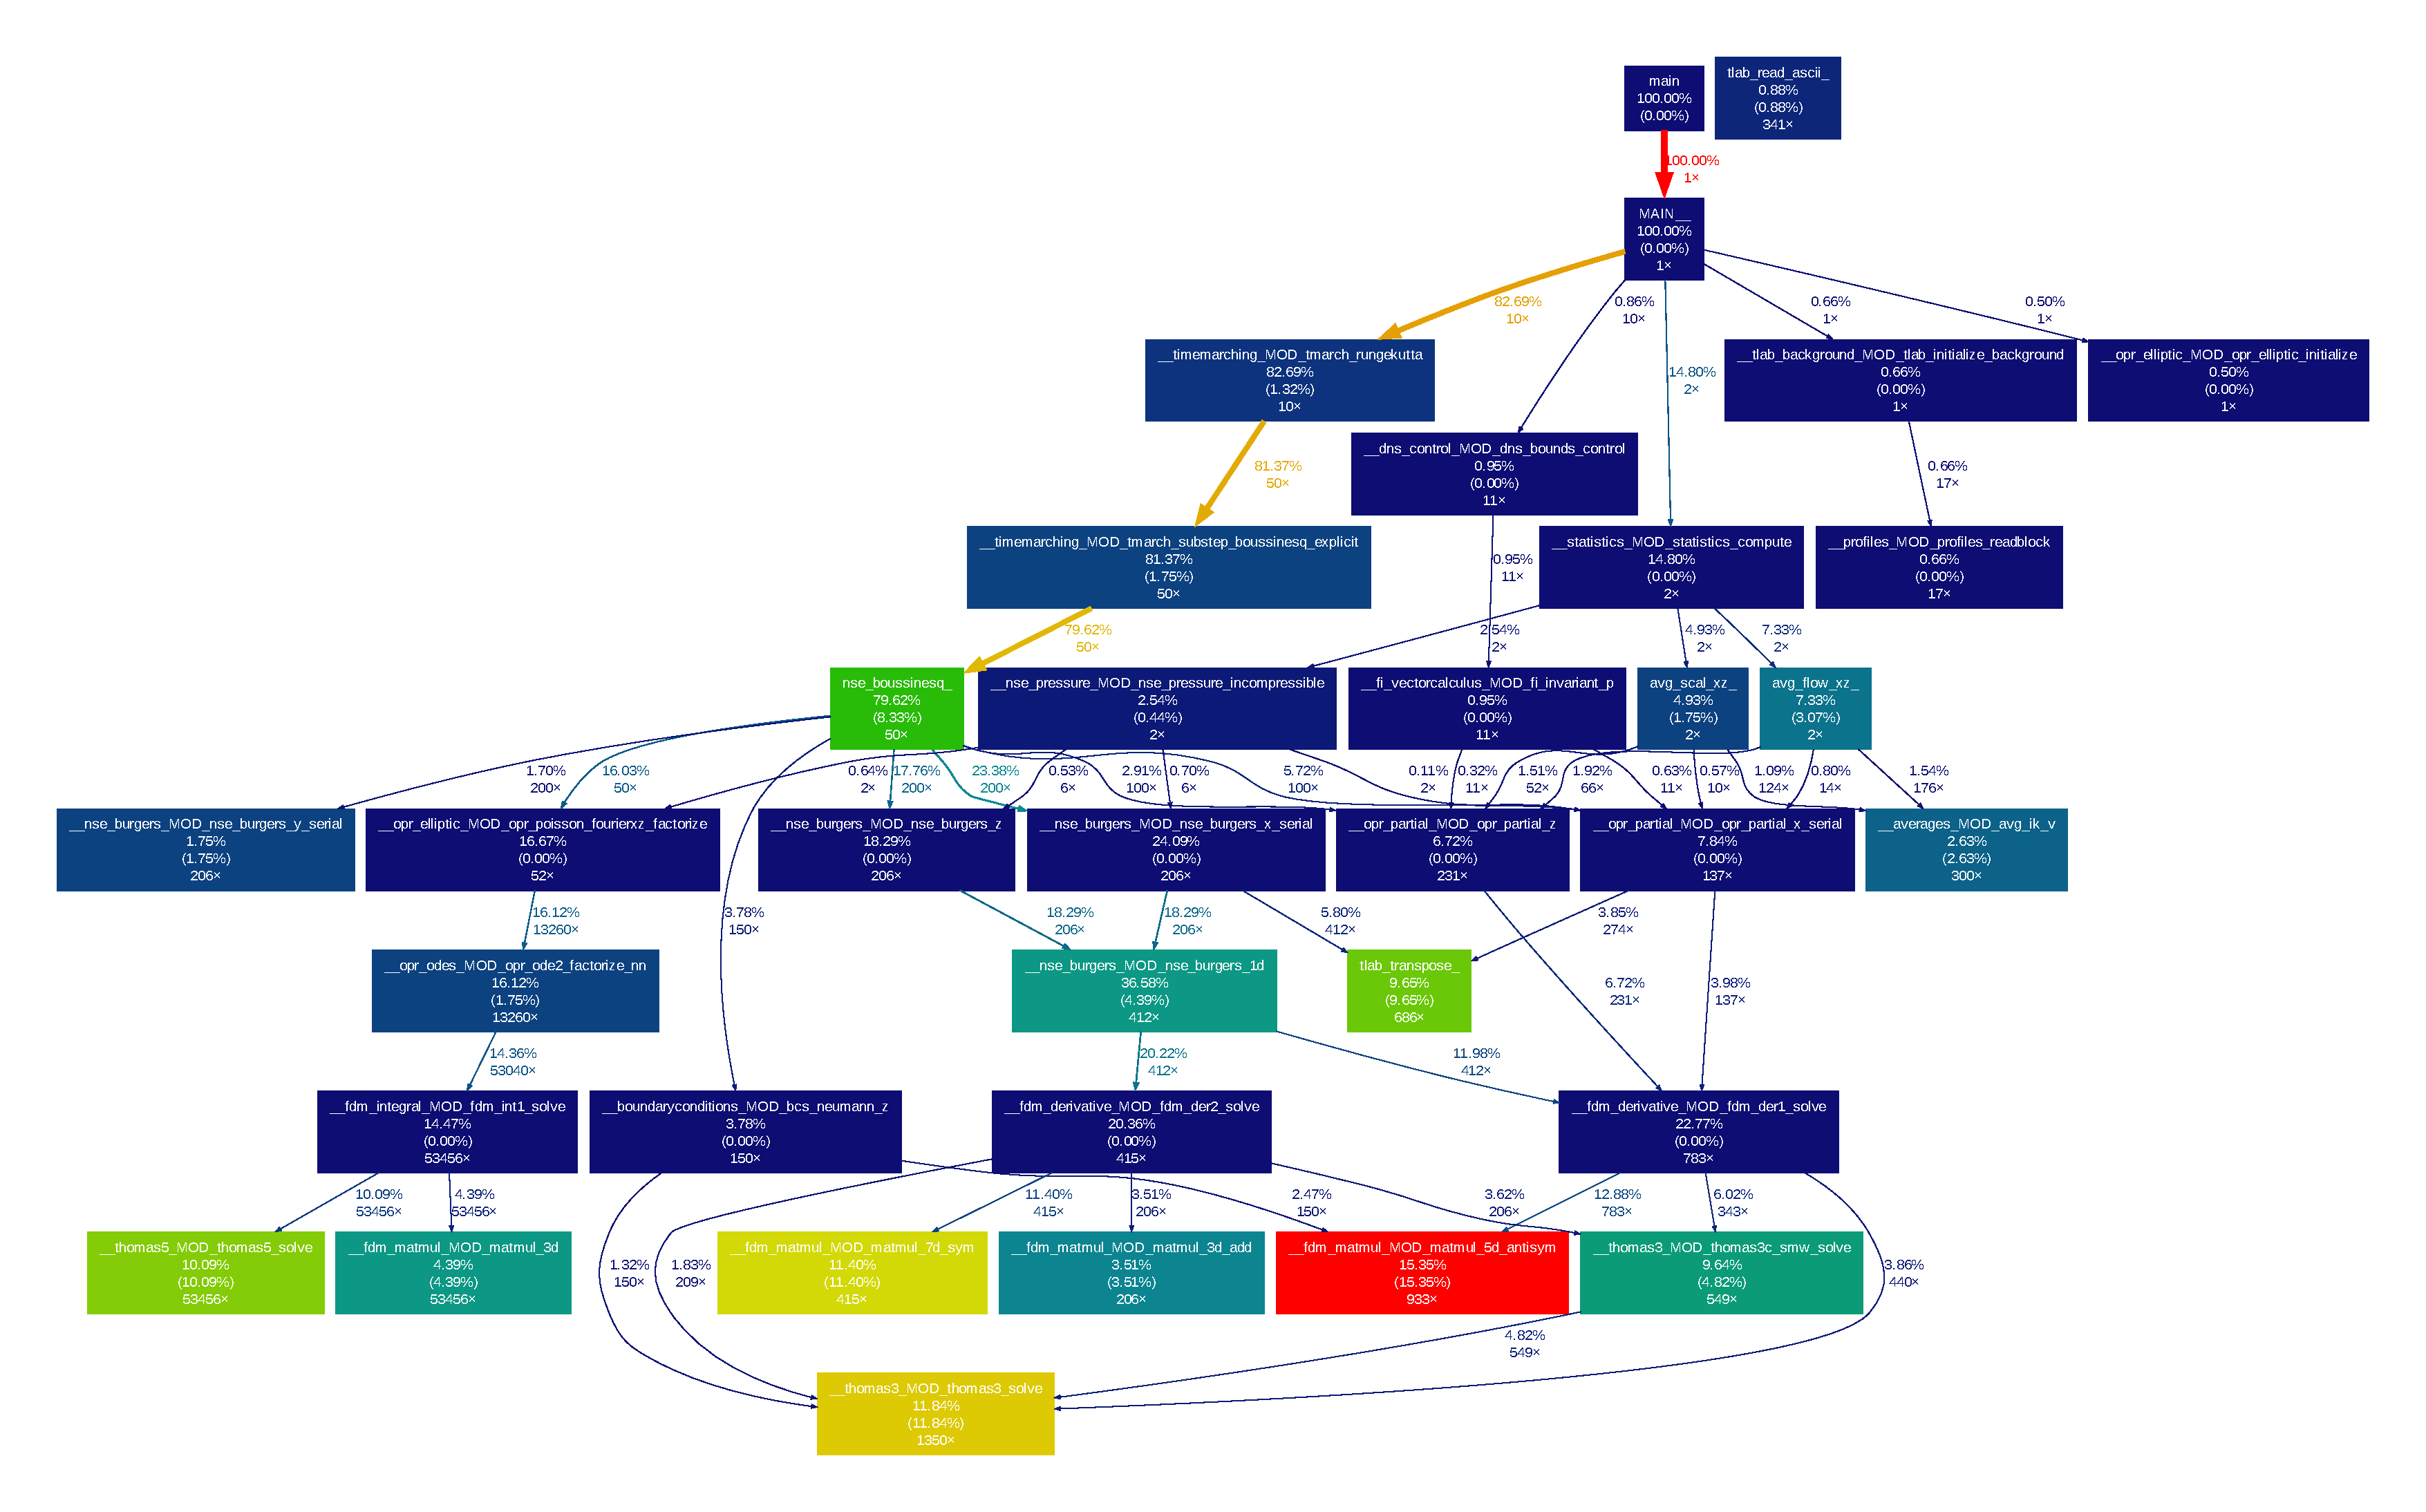
\includegraphics[clip,width=\textwidth]{fig-profiling08.pdf}
  \caption{Profiling diagram of \texttt{examples/Case08} running 50 iterations in serial mode.}
\end{figure}

\newpage

\begin{figure}[!h]
  \centering
  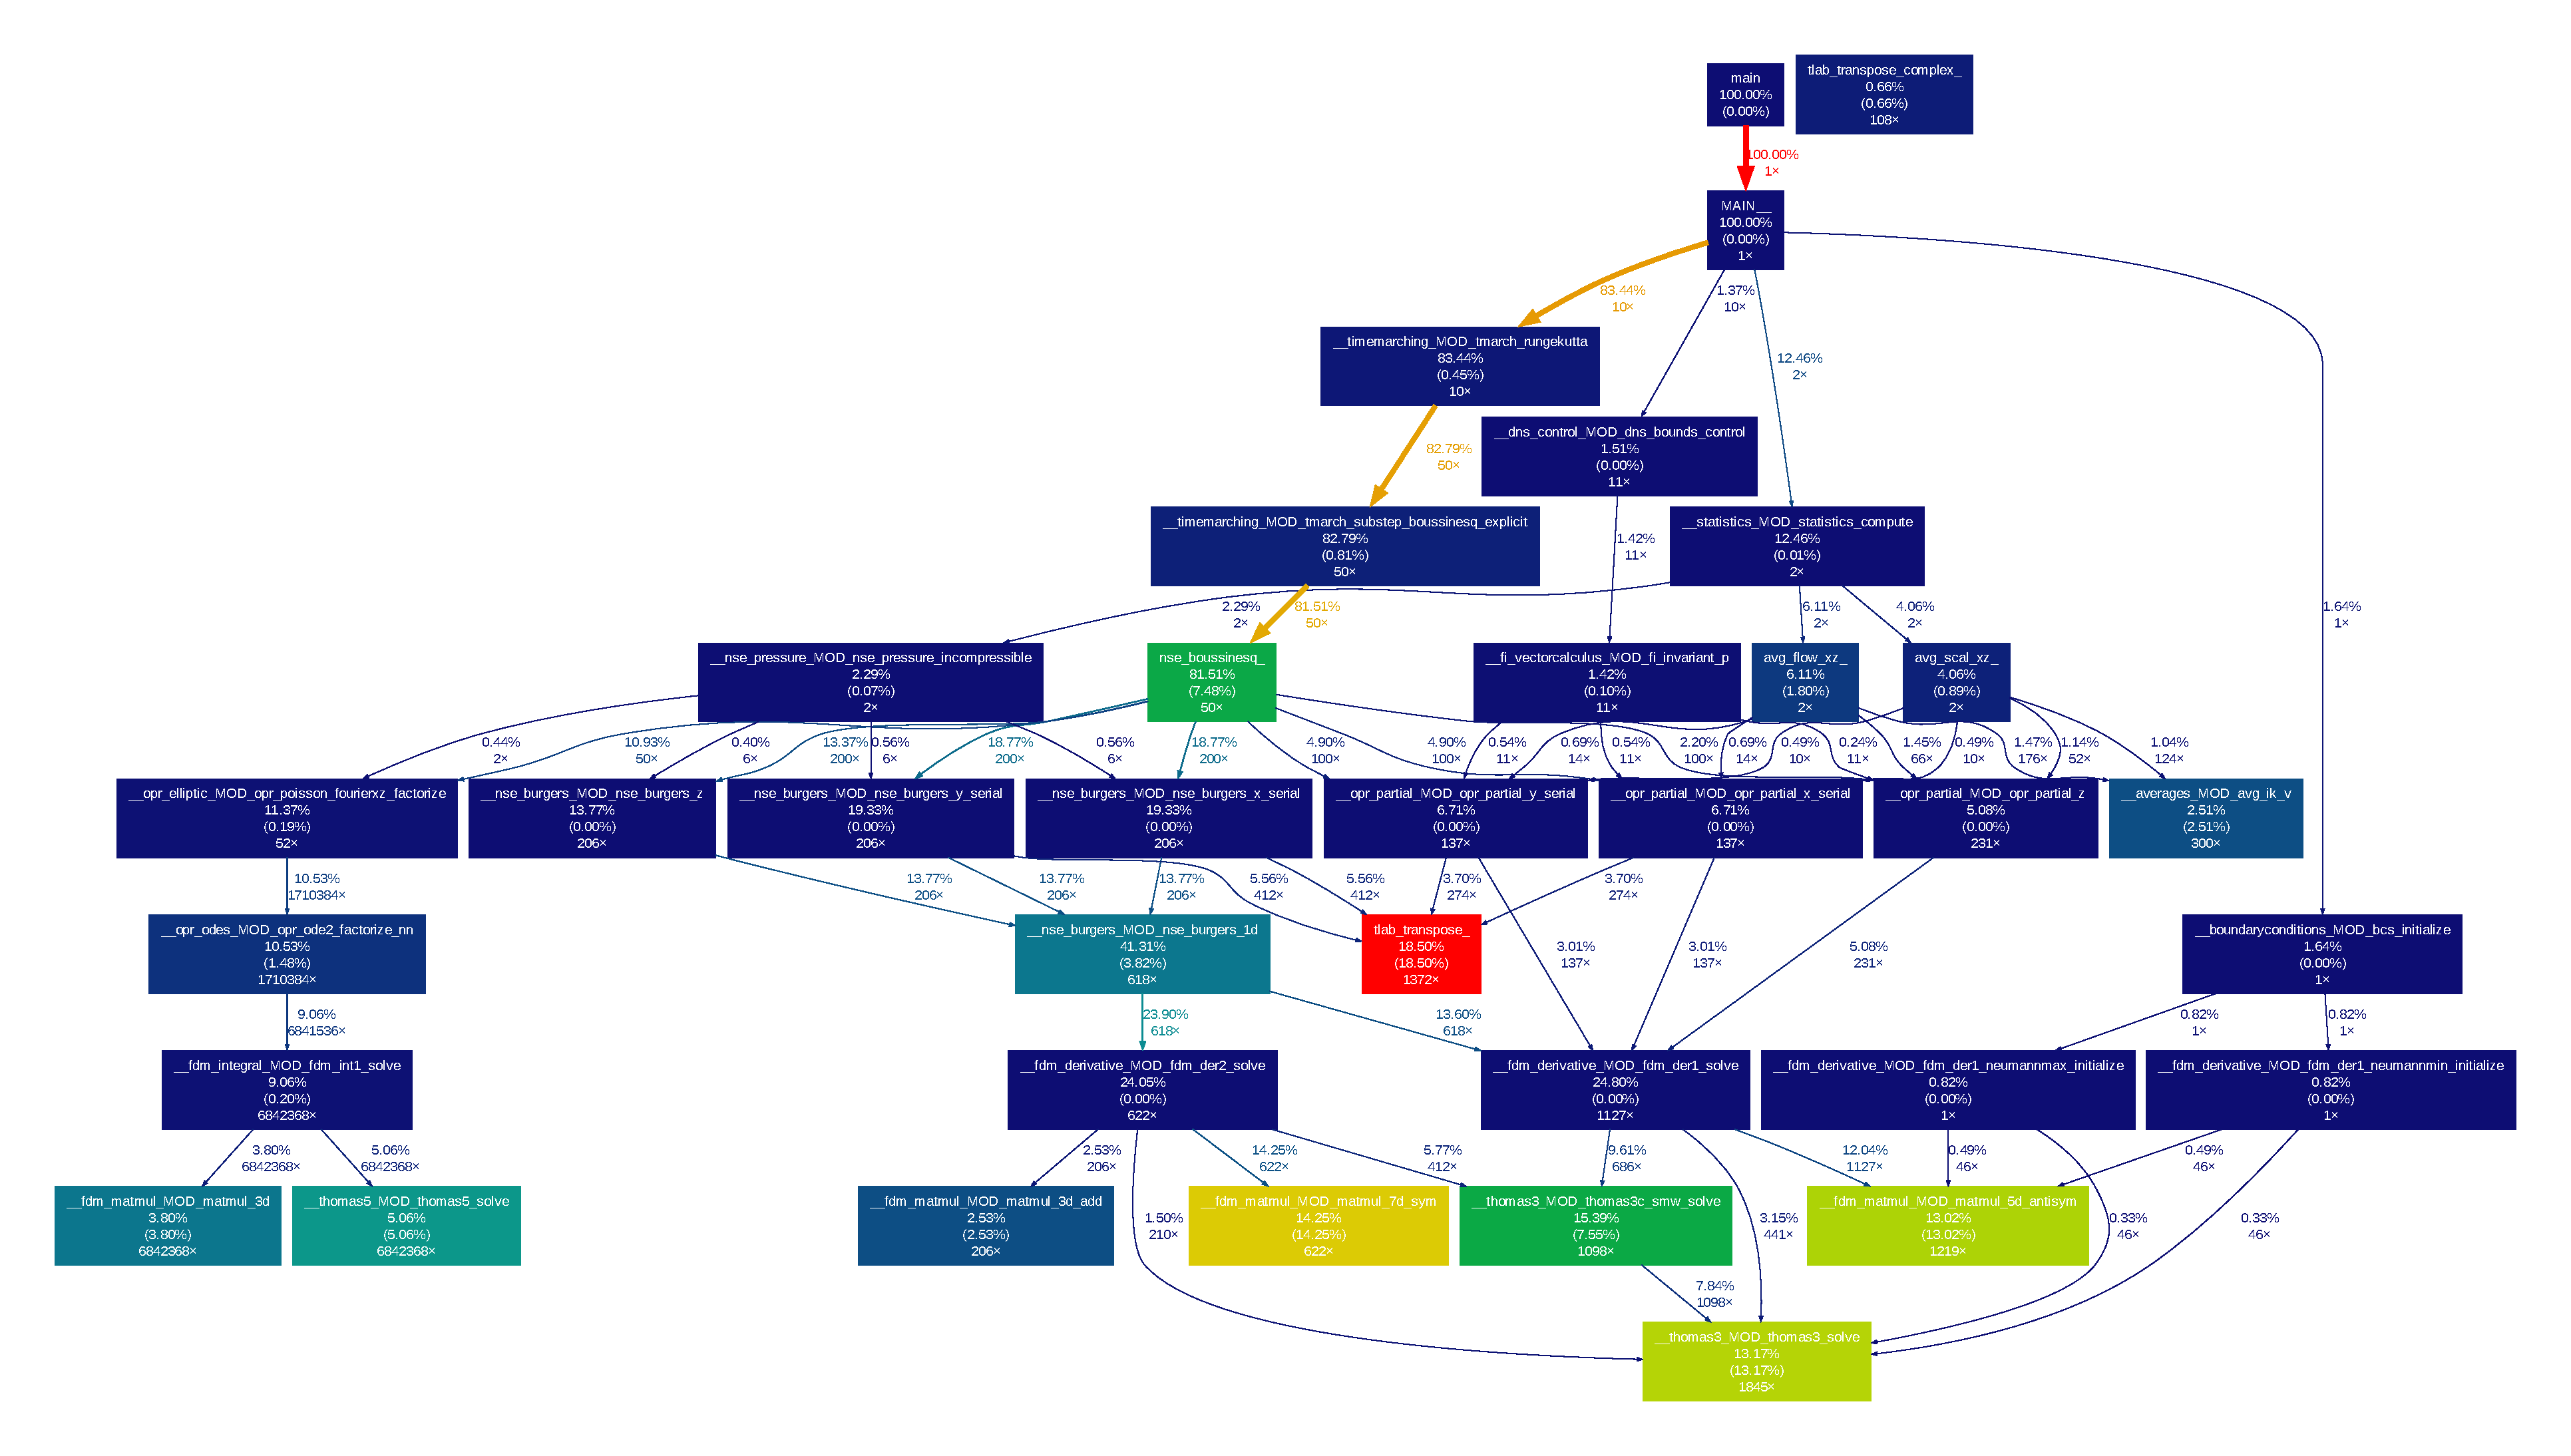
\includegraphics[clip,width=\textwidth]{fig-profiling08-3d.pdf}
  \caption{Profiling diagram of \texttt{examples/Case08-3d} running 50 iterations in serial mode.}
\end{figure}

% \newpage

\begin{figure}[!h]
  \centering
  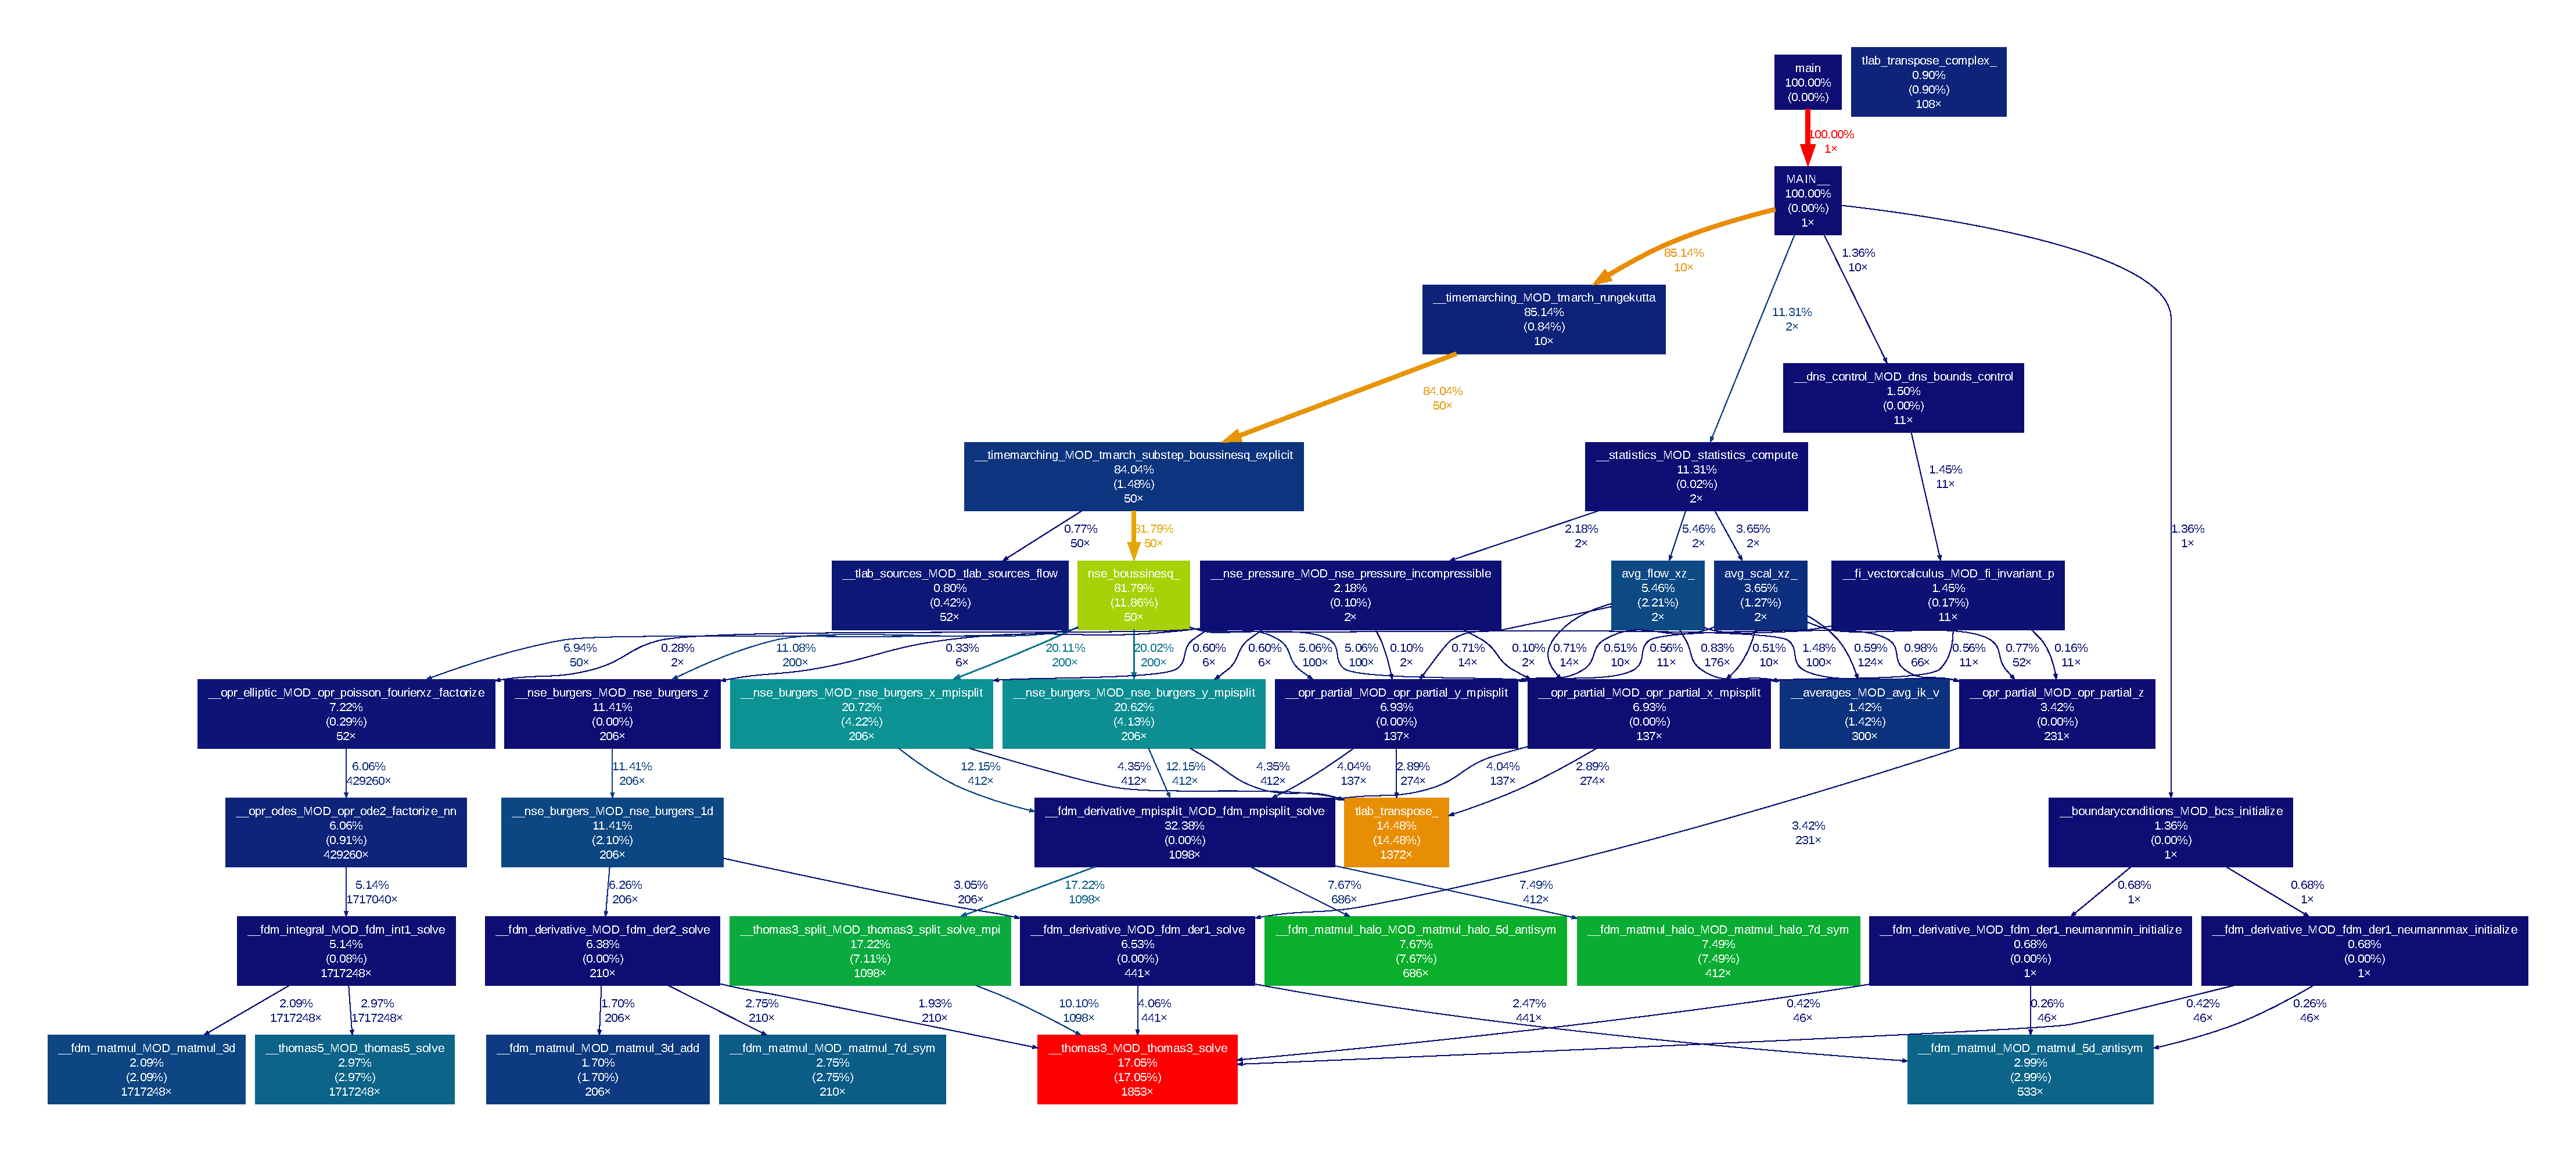
\includegraphics[clip,width=\textwidth]{fig-profiling08-3d-mpi.pdf}
  \caption{Profiling diagram of \texttt{examples/Case08-3d} running 50 iterations in parallel mode with 4 processors.}
\end{figure}

\newpage

\begin{figure}[!h]
  \centering
%   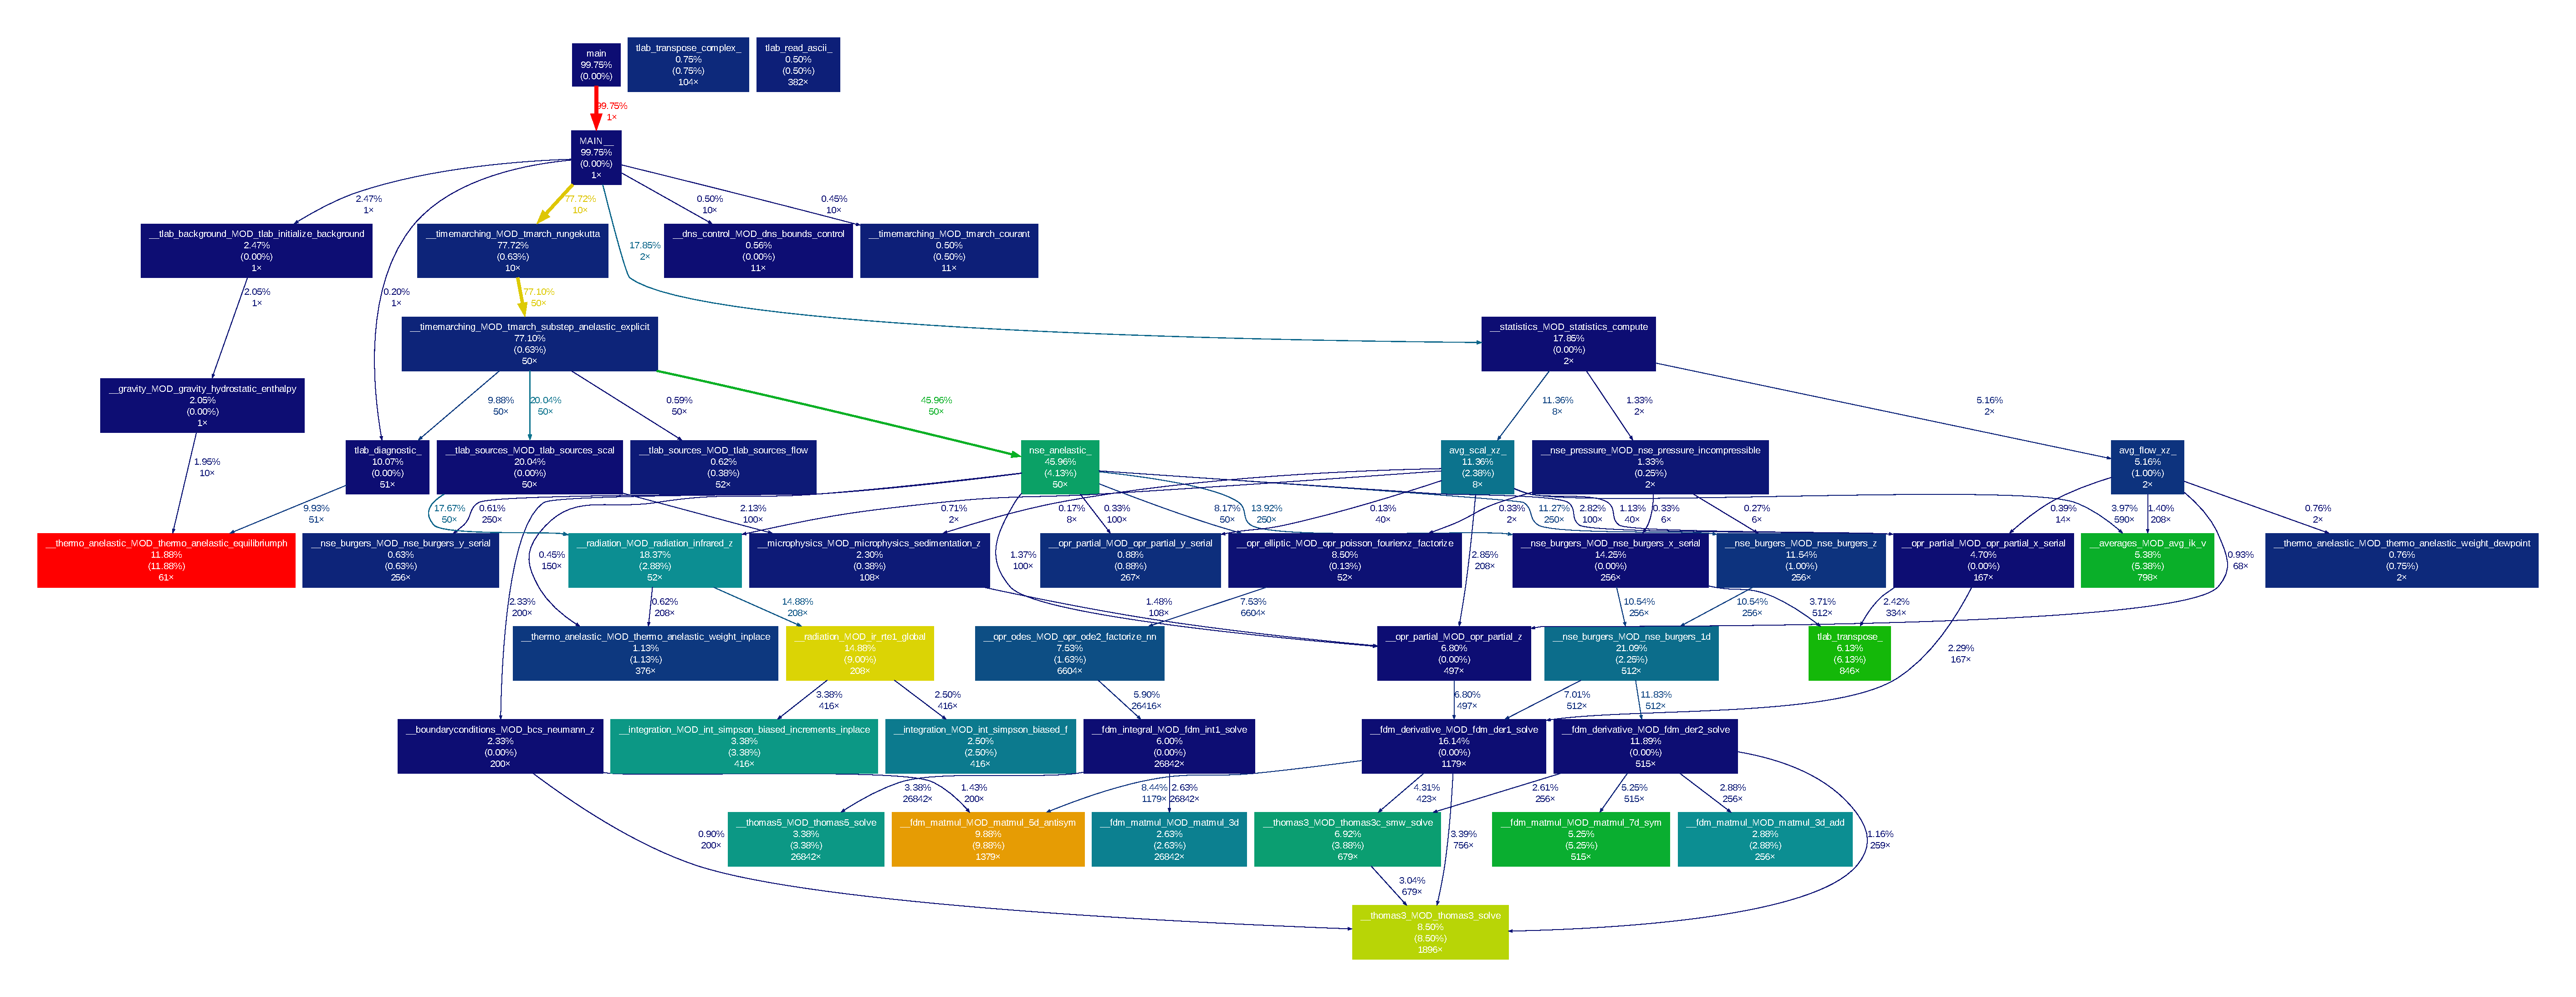
\includegraphics[clip,width=0.9\textheight,angle=90]{fig-profiling65.pdf}
  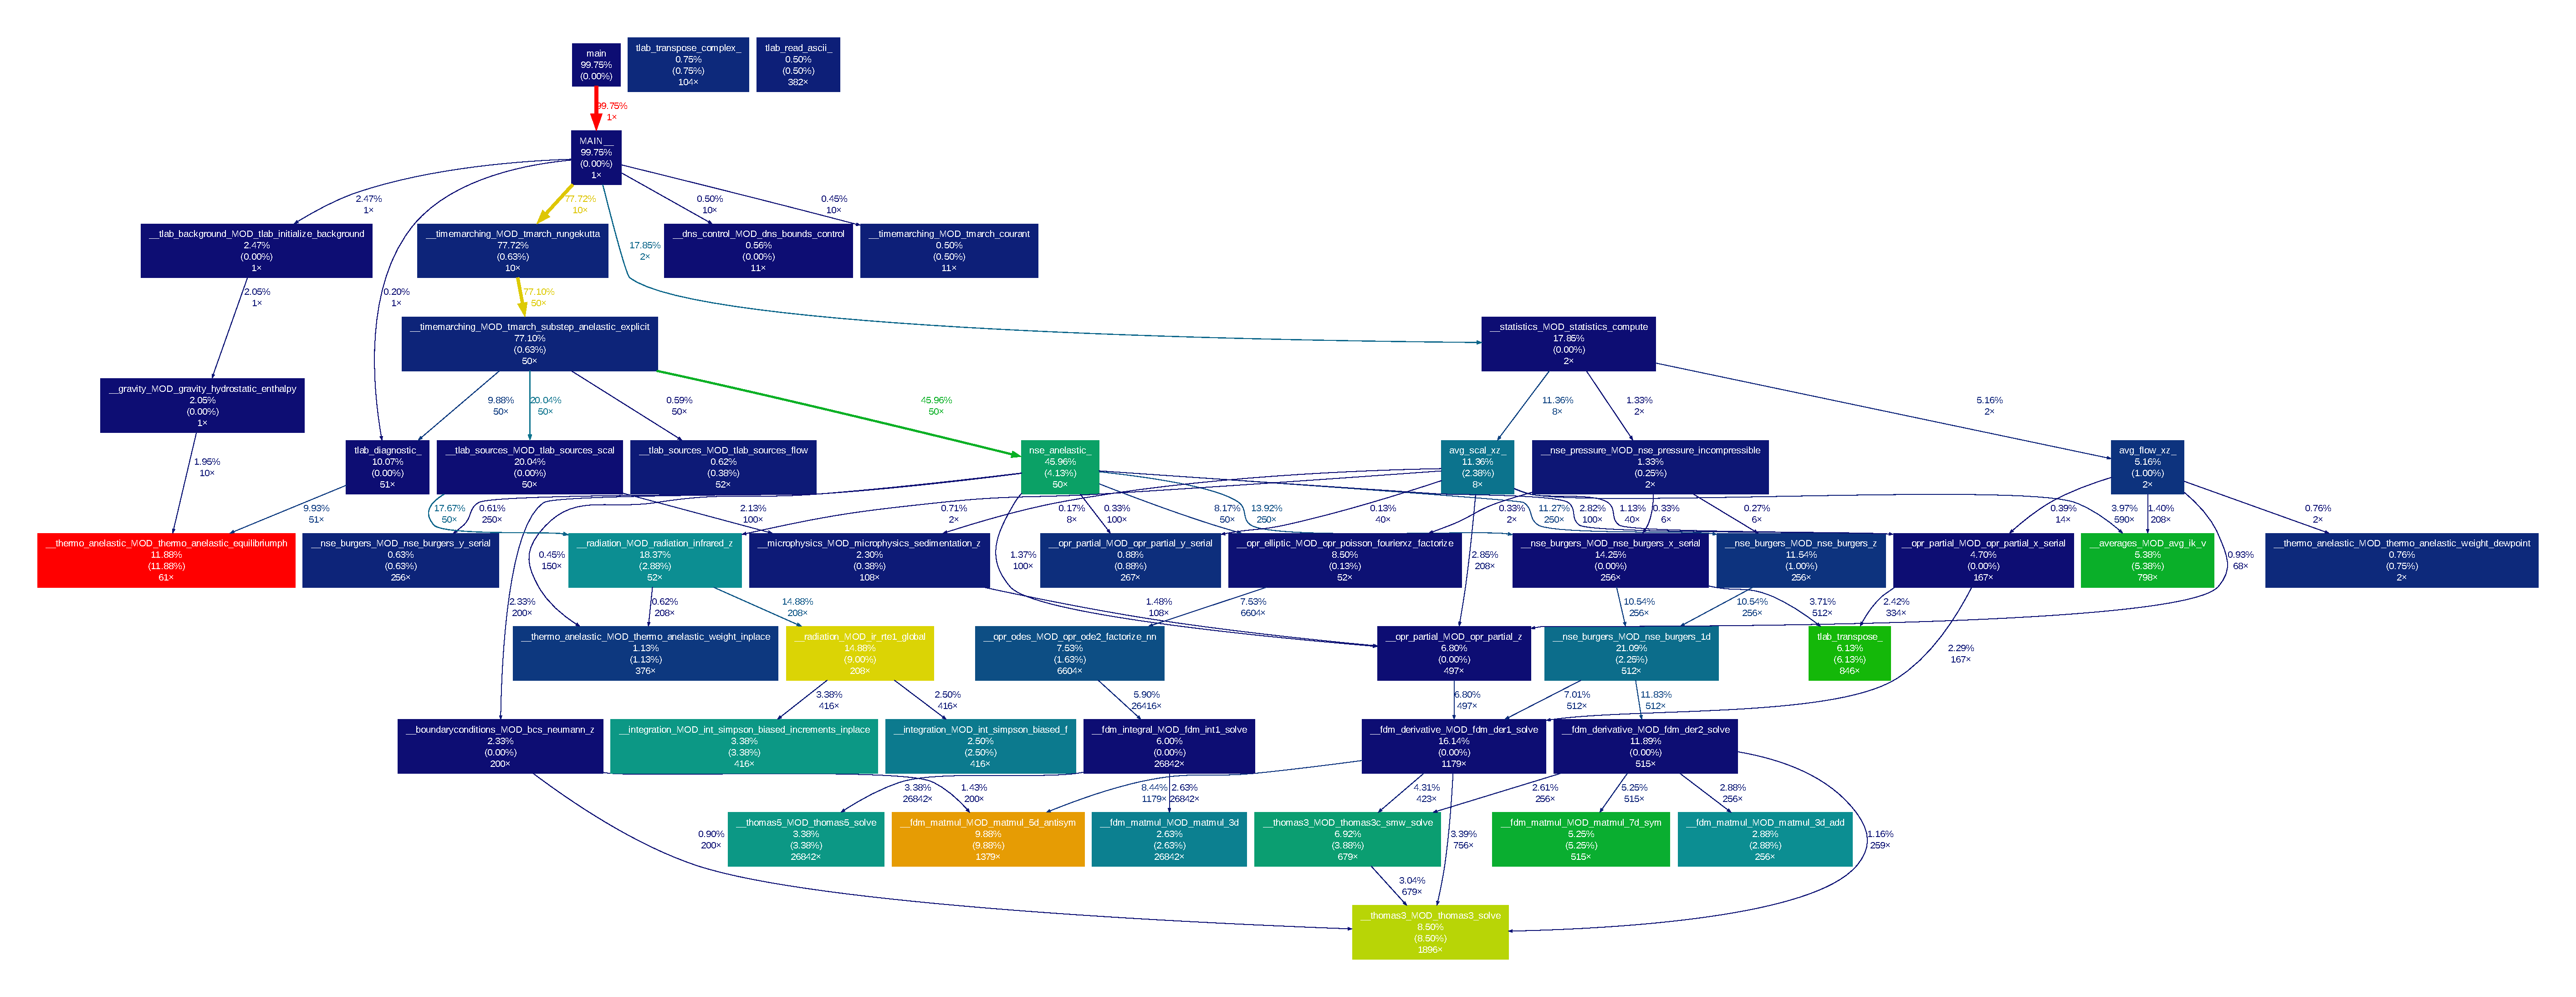
\includegraphics[clip,width=\textwidth]{fig-profiling65.pdf}
  \caption{Profiling diagram of \texttt{examples/Case65} running 50 iterations in serial mode.}
\end{figure}

% \caption{Profiling diagram of modified \texttt{examples/Case44} (768 cube) running 25 iterations in parallel mode with 48 tasks (1 node on juwels).}


\backmatter
\bibliographystyle{plainnat}
\bibliography{atlab-doc.bib}

\end{document}
